\documentclass[11pt]{article}
\usepackage[utf8]{inputenc}
\usepackage{float}
\usepackage{amsmath}
\usepackage{tikz} % for Hasse diagram
\usepackage[hmargin=3cm,vmargin=6.0cm]{geometry}
%\topmargin=0cm
\topmargin=-2cm
\addtolength{\textheight}{6.5cm}
\addtolength{\textwidth}{2.0cm}
%\setlength{\leftmargin}{-5cm}
\setlength{\oddsidemargin}{0.0cm}
\setlength{\evensidemargin}{0.0cm}

\begin{document}
	
\section*{Student Information } 
%Write your full name and id number between the colon and newline
%Put one empty space character after colon and before newline
Full Name :  Adil Kaan Akan \\
Id Number :  2171155\\

% Write your answers below the section tags
\section*{Answer 1}
By the  handshaking theorem, we know that a graph G=(V,E) has a property which is sum of degrees of all nodes equals to two times of number of edges. That is, $2*e = \sum\limits_{v \in V}{degree(v)}$.

We know that the number of edges is 23 and all nodes have at least degree 4.Then, by the theorem \\
	
\begin{align*}	
	2*e &= \sum\limits_{v \in V}{degree(v)} \\
	2*23 &= \sum\limits_{v \in V}{degree(v)} \\
\end{align*}
Then, in order to have maximum number of nodes we need the all nodes with minumum degree. That is 4. Then, \\

\begin{align*}	
	2*e &= \sum\limits_{v \in V}{degree(v)} \\
	2*23 &= |V|*4 \\
	46 &= |V|*4 \\
\end{align*}
Then, the integer part of $|V|$ is 11. Then, we have the maximum number of nodes that is 11. \\




\section*{Answer 2}
We can prove that with adding one vertex V  to a graph G and connecting all vertices to V. When we add an vertex to the graph G, we have graph with min degree $\frac{n-1}{2} + 1$. We know that Dirac's theorem states that any simply connected graph with three or more vertex n  with degree greater than $\frac{n}{2}$ has hamiltonian cycle. When we add an vertex to graph G, we had degree $\frac{n-1}{2} + 1$ that is greater than 
$\frac{n}{2}$. Since the graph G has at least 5 vertex and has a degree which is $\frac{n+1}{2}$, the graph G has hamiltonian cycle which includes our vertex V. Removing V and all edges that we connect breaks the cycle but leaves hamiltonian path. Then, our proof will be true.


\section*{Answer 3}
Bipartite graph means that set of vertices decomposed into two disjoint sets and there is no edge in between vertices that are in same set. That is, no two vertices within the same set are adjacent.If the vertices taken in order, that is first picked from one set and second picked from other set and it goes on, adjancency matrix of a bipartite graph has blocks in itself. \\

\begin{align*}
M = \begin{pmatrix} 0 & B \\ B^T & 0 \end{pmatrix}
\end{align*}

Then, if we multiply M by itself \\

\begin{align*}
M^2=\begin{pmatrix}
0 & B \\ B^T & 0
\end{pmatrix}\begin{pmatrix}
0 & B \\ B^T & 0
\end{pmatrix}=\begin{pmatrix}
BB^T & 0 \\ 0 & B^TB
\end{pmatrix}
\end{align*}

And one more, \\

\begin{align*}
M^3=\begin{pmatrix}
BB^T & 0 \\ 0 & B^TB
\end{pmatrix}\begin{pmatrix}
0 & B \\ B^T & 0
\end{pmatrix}=\begin{pmatrix}
0 & BB^TB \\ B^TB & 0
\end{pmatrix}
\end{align*}

And it goes on like that, on even powers of M diagonal entries are not zero, but on odd power of M diagonal entries will be zero.  \\

\section*{Answer 4}
\subsection*{a.}
In Kruskal's algorithm we place nodes first, then we choose edge with minumum weight. Table shows that choices.
\begin{table}[H]
\centering
\caption{Table for kruskal algorithm}
\label{a.}
\begin{tabular}{|l|l|l|}
\hline
 Choice & Edge  & Weight  \\ \hline
 1& (e-f) & 1 \\ \hline
 2& (e-h) & 2 \\ \hline
 3& (g-h) &  2\\ \hline
 4& (a-d) & 2 \\ \hline
 5& (d-g) & 3 \\ \hline
 6& (d-b) &  3\\ \hline
 7& (c-f) &  3\\ \hline
 8& (h-i) & 4 \\ \hline
\end{tabular}
\end{table}



\subsection*{b.}

We can start the algorithm by randomly choosing e as a starting vertex. Then, the table shows the choices of edges.
\begin{table}[H]
\centering
\caption{Table for Prim's algorithm}
\label{b.}
\begin{tabular}{|l|l|l|}
\hline
 Choice & Edge  & Weight  \\ \hline
1 & (e-f) & 1 \\ \hline
 2& (e-h) & 2 \\ \hline
3 & (h-g) &  2\\ \hline
 4& (f-c) & 3 \\ \hline
 5& (g-d) & 3 \\ \hline
 6& (d-a) &  2\\ \hline
 7& (d-b) &  3\\ \hline
 8& (h-i) & 4 \\ \hline
\end{tabular}
\end{table}

\begin{figure}[H]	\caption{ Delete the related edges to display the acquired MST}
	\centering
	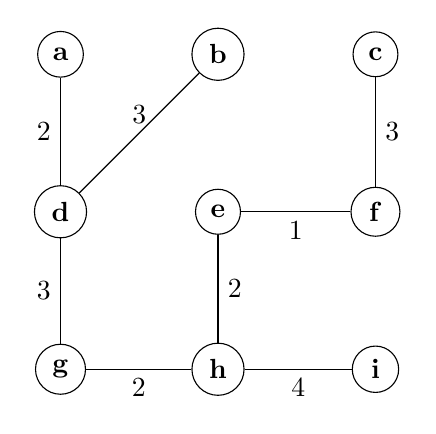
\begin{tikzpicture}
	
	\node[shape=circle,draw=black] (a) at (0, 4)     {\textbf{a}};
	\node[shape=circle,draw=black] (b) at (2, 4)     {\textbf{b}};
	\node[shape=circle,draw=black] (c) at (4, 4)     {\textbf{c}};
	\node[shape=circle,draw=black] (d) at (0, 2)     {\textbf{d}};
	\node[shape=circle,draw=black] (e) at (2, 2)     {\textbf{e}};
	\node[shape=circle,draw=black] (f) at (4, 2)     {\textbf{f}};
	\node[shape=circle,draw=black] (g) at (0, 0)     {\textbf{g}};
	\node[shape=circle,draw=black] (h) at (2, 0)     {\textbf{h}};
	\node[shape=circle,draw=black] (i) at (4, 0)     {\textbf{i}};
	
	
	\path[-] (a) edge  node[left]  {2} (d);
	\path[-] (b) edge  node[above] {3} (d);
	\path[-] (c) edge  node[right] {3} (f);
	\path[-] (d) edge  node[left]  {3} (g);
	\path[-] (e) edge  node[below] {1} (f);
	\path[-] (e) edge  node[right] {2} (h);
	\path[-] (g) edge  node[below] {2} (h);
	\path[-] (h) edge  node[below] {4} (i);
	
	\end{tikzpicture} 
\end{figure}

\end{document}